
%(BEGIN_QUESTION)
% Copyright 2013, Tony R. Kuphaldt, released under the Creative Commons Attribution License (v 1.0)
% This means you may do almost anything with this work of mine, so long as you give me proper credit

Examine this right triangle (a triangle with one 90$^{o}$ angle), and identify which side is the opposite, the adjacent, and the hypotenuse as viewed from two different angles ($a$ and $b$):

$$\includegraphics[width=15.5cm]{i02648x01.eps}$$

\noindent
As viewed from angle $a$:

\item{} Opposite side = \underbar{\hskip 50pt}
\item{} Adjacent side = \underbar{\hskip 50pt}
\item{} Hypotenuse side = \underbar{\hskip 50pt}
\end{itemize}

\vskip 10pt

\noindent
As viewed from angle $b$:

\item{} Opposite side = \underbar{\hskip 50pt}
\item{} Adjacent side = \underbar{\hskip 50pt}
\item{} Hypotenuse side = \underbar{\hskip 50pt}
\end{itemize}

\underbar{file i02648}
%(END_QUESTION)





%(BEGIN_ANSWER)

\noindent
As viewed from angle $a$:

\item{} Opposite side = \underbar{$Y$}
\item{} Adjacent side = \underbar{$Z$}
\item{} Hypotenuse side = \underbar{$X$}
\end{itemize}

\vskip 10pt

\noindent
As viewed from angle $b$:

\item{} Opposite side = \underbar{$Z$}
\item{} Adjacent side = \underbar{$Y$}
\item{} Hypotenuse side = \underbar{$X$}
\end{itemize}


\vskip 10pt

Imagine the triangle being a room, viewed from above, with you standing at the location of the angle in question.  The hypotenuse is {\it always} the longest of the three sides in a right triangle, regardless of which angle is being considered.  The {\it adjacent} side is the non-hypotenuse side that you can reach from where you stand (i.e. the side that is ``adjacent to'' or ``next to'' the angle).  The {\it opposite} side is the non-hypotenuse side that you can see on the other side of the room from your location (i.e. the side that is ``opposite'' the angle).

$$\includegraphics[width=15.5cm]{i02648x02.eps}$$

%(END_ANSWER)





%(BEGIN_NOTES)


%INDEX% Mathematics review: trigonometric calculations

%(END_NOTES)


